\chapter{Le framework Mechanics, Dynamics, Aesthetics}



\section{L'origine du framework}
[MDA article]
La particularité du développement de jeux vidéos est que sa consommation n'est pas prévisible
Le MDA peut etre vu comme des lenses

[Leblanc ppt]
\begin{figure}[H]
    \centering
    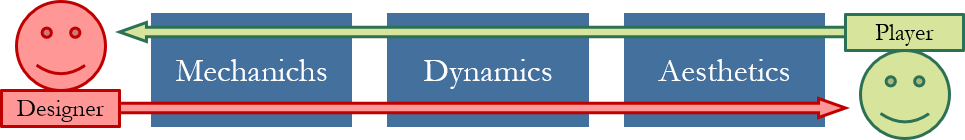
\includegraphics[width=10cm]{10_img/chap3/desvspla.png} 
    \caption{Perspective des Designer VS perspective des Joueurs \cite{MDA_formal}}
\end{figure}
Différence entre une appli et un jeu : 
- un user apporte un but a une appli (l'app repond à un besoin du user)
- Un jeu apporte un but à un joueur (c'est le jeu qui est acteur du but)

\begin{figure}[H]
    \centering
    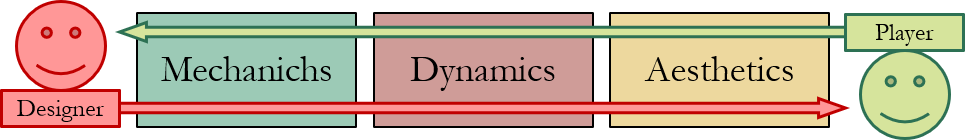
\includegraphics[width=14cm]{10_img/chap3/mda.png} 
    \caption{Contenu des parties du Framework MDA \cite{MDA_formal}}
\end{figure}


%MDA: A Formal Approach to Game Design and Game Research Robin Hunicke, Marc LeBlanc, Robert Zubek
%A better recipe for game jams: using the Mechanics Dynamics Aesthetics framework for planning Paris Buttfield-Addison,Jon Manning,Tim Nugent
%\Design, Dynamics, Experience (DDE): An Advancement of the MDA Framework for Game Design
\section{Mechanics}
[Leblanc ppt] Mechanics = code + rules / Game as system
Représentation des datas et algorithmes
Tous les objets et les mécaniques de jeux (level design, gameplay...).
Toutes les actions, comportements et controles attribués au joueur.
Il existe beaucoup de méchanics de jeu (cards, shooter, golf...)
Certains comportement sont des conséquences directes des règles = mechanics


\section{Dynamics}
[Leblanc ppt] Dynamics Process + Game "session"
Mechanics et Dynamics sont différentes view du jeu
Les Dynamics découlent des Mechanics
Certains comportement sont des conséquences indirectes des règles = Dynamics
Comportement au runtime
Partie des mechanics que le joueur peut voir: qu'est ce qu'il se passe quand le joueur appuie sur un bouton, qu'est ce qu'il se passe quand il effectue une action 
Qu'est ce qui est prédictible et explicable concernant le comportement du jeu ?
Il est possible d'analyser les autres jeux mais également : utiliser les calculs des autres jeux (maths), étudier la psychologie du joueur...


\section{Aesthetics}
[Leblanc ppt] Aesthetics Requirements + fun
représente les émotions générées pour le joueur quand il intéragit avec le systeme
Passe par tous les sens atteignables et les émotions
8 sortes de "fun"(Jeu pour le) : sensation (plaisir des sens), fantasy (make-believe), narrative(drama), challenge(suite d'obstacles), fellowship(réseau social), discovery(territoires inconnus), expression(découverte de soi meme), submission(passe temps).
Chaque jeu peut contenir un ou plusieurs types de fun
L'aesthetics peut etre un objectif dans le développement d'un jeu

\section{Les limitations et évolutions possibles}
%ARTCILE The Design, Play, and Experience Framework, Brian M. Winn
DPE (Design Play Experience framework pour designer les serious games
Approche formelle pour diesigner l'apprentissage, le story telling, le gameplay, l'experience utilisateur et les composants techno d'un jeu sérieux
DPE est une extension du MDA

\begin{figure}[H]
    \centering
    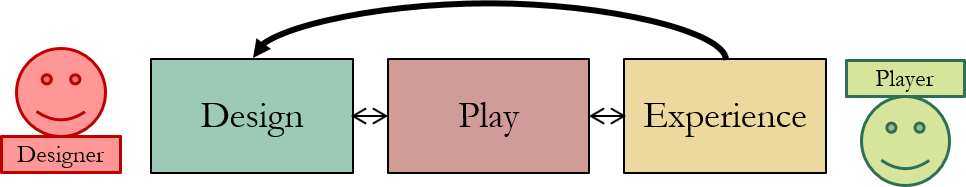
\includegraphics[width=10cm]{10_img/chap3/dpe.png} 
    \caption{Contenu des parties du Framework DPE \cite{Winn2011}}
\end{figure}

Le designer design le jeu, le joueur y joue, ce qui créé l'expérience.
Le designer a le contrôle direct sur tout le design. Pour cela il doit définir des objectifs d'expérience (c'est ce que représente la flèche depuis Experience vers Design). Cette flèche représente aussi le processus itératif du design (Salen et Zimmermann 2004) Le design entraîne un prototype, l'expérience sur ce prototype permet de revoir le design.



\begin{figure}[H]
    \centering
    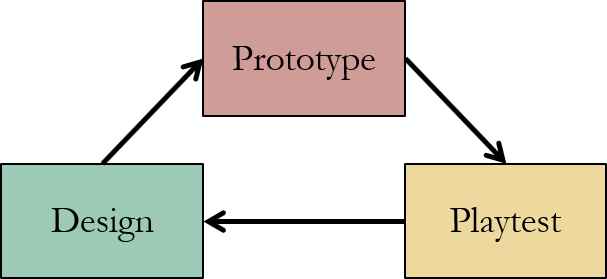
\includegraphics[width=8cm]{10_img/chap3/iteration_prototype.png} 
    \caption{Processus de design itératif \cite{Winn2011}}
\end{figure}

\begin{figure}[H]
    \centering
    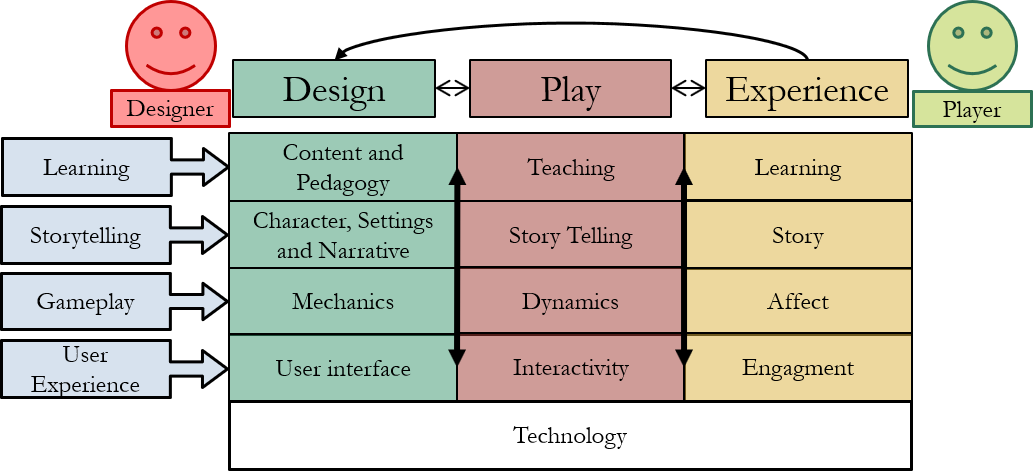
\includegraphics[width=14cm]{10_img/chap3/dpe_extended.png} 
    \caption{Framework DPE étendu \cite{Winn2011}}
\end{figure}



%ARTICLE DDE Design, Dynamics, Experience (DDE): An Advancement of the MDA framework for Game Design Wolfgang
Néglige beaucoup d'aspects de design des jeux vidéos
Se concentre trop sur les méacaniques
Ne convient pas à tous les types de gameplay (jeux sérieux, gamification, narrative
Schell introduit des notions de Story et Technologies, alliées à la méecanique et aesthetics du MDA. 
Dans le MDA le designer n'a que peu de controle sur les dynamics et aesthetics car ceux ci decoulent que des mecaniques décrites avant.


\begin{figure}[H]
    \centering
    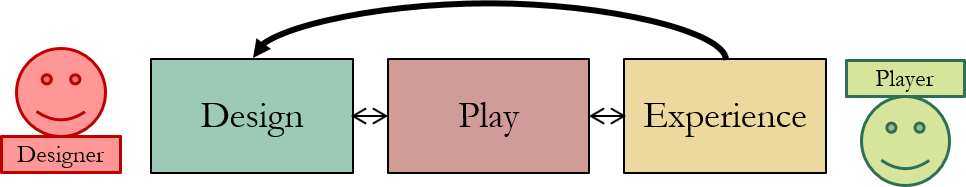
\includegraphics[width=10cm]{10_img/chap3/dpe.png} 
    \caption{Contenu du Framework DDE \cite{DDE}}
\end{figure}

\begin{figure}[H]
    \centering
    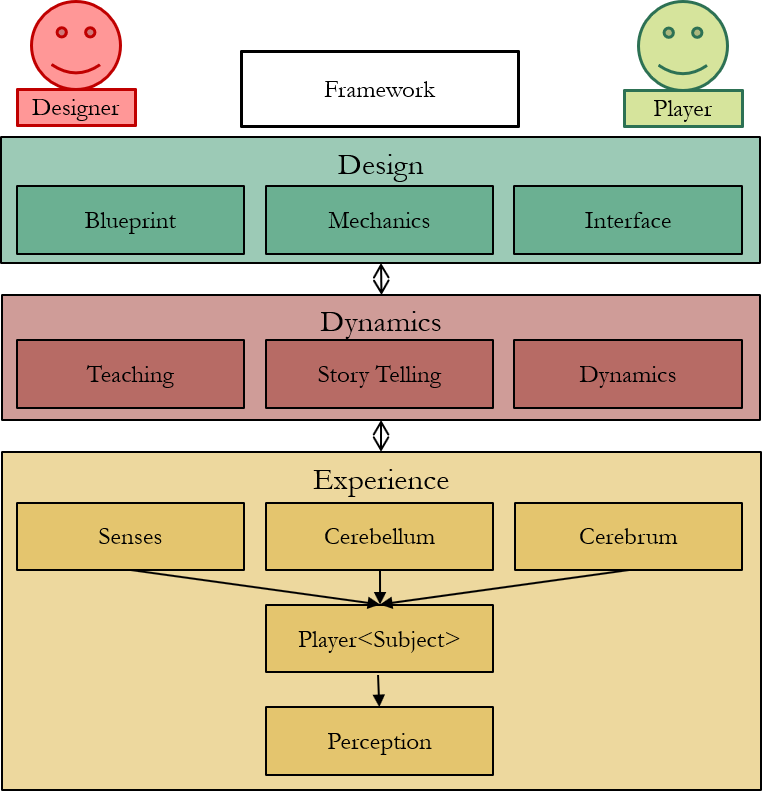
\includegraphics[width=14cm]{10_img/chap3/dde_extended_modif.png} 
    \caption{Framework DDE étendu \cite{DDE}}
\end{figure}
%GAMASUTRA Revisiting the MDA framework, Luiz Claudio Silveira Duarte
%GAMASUTRA From MDA to DDE, Wolfgang Walk